%!TEX root = da-dev.tex

In Section~\ref{sec:intro-neg-logstar}, we gave a proof of the following result: in the $\LOCAL$ model, it is not possible to find a $3$-colouring of a directed cycle in $O(1)$ rounds with deterministic algorithms. In this chapter, we will give another proof of the same result, this time with the help of Ramsey's theorem (recall Chapter~\ref{ch:ramsey}). In the exercises, we will see plenty of other applications of Ramsey's theorem in this context, some of which would be rather difficult to prove with the technique that we used in Section~\ref{sec:intro-neg-logstar}.


\section{Claim}

We will prove the following theorem.

\begin{theorem}\label{thm:colour-lb}
    Assume that $A$ is a deterministic distributed algorithm for the $\LOCAL$ model. Assume that there is a constant $T \in \NN$ such that $A$ stops in time $T$ in any directed cycle $G = (V,E)$, and outputs a labelling $g\colon V \to \{1,2,3\}$. Then there exists a directed cycle $G$ and an assignment of unique identifiers such that if we execute $A$ on $G$, the output of $A$ is not a proper vertex colouring of~$G$.
\end{theorem}


\section{Preliminaries}

To prove Theorem~\ref{thm:colour-lb}, let $n = 2T+2$, $k = 2T+1$, and $c = 3$. By Ramsey's theorem, $R_c(n;k)$ is finite. Choose any $N \ge R_c(n;k)$.

We will construct a directed cycle $G = (V,E)$ with $N$ nodes. In our construction, the set of nodes is $V = \{1,2,\dotsc,N\}$. This is also the set of unique identifiers in our cycle; recall that we follow the convention that the unique identifier of a node $v \in V$ is $v$.

With the set of nodes fixed, we proceed to define the set of edges. In essence, we only need to specify in which order the nodes are placed along the cycle.


\section{Subsets and Cycles}

For each subset $X \subseteq V$, we define a directed cycle $G_X = (V,E_X)$ as follows; see Figure~\ref{fig:subset-cycle}. Let $\ell = |X|$. Label the nodes by $x_1, x_2, \dotsc, x_N$ such that
\begin{align*}
    X &= \Set{ x_1, x_2, \dotsc, x_{\ell} }, \\
    V \setminus X &= \Set{ x_{\ell+1}, x_{\ell+2}, \dotsc, x_N }, \\
    x_1 &< x_2 < \dotsb < x_{\ell}, \\
    x_{\ell+1} &< x_{\ell+2} < \dotsb < x_N.
\end{align*}
Then choose the edges
\[
    E_X = \Set{ (x_i, x_{i+1}) : 1 \le i < N } \, \cup \, \Set{ (x_N,x_1) }.
\]

\begin{figure}
    \centering
    \includegraphics[page=\PSubsetCycle]{figs.pdf}
    \caption{Construction of $G_X$. Here $N = 6$ and $X = \{2,4\}$.}\label{fig:subset-cycle}
\end{figure}

Informally, $G_X$ is constructed as follows: first take all nodes of $X$, in the order of increasing identifiers, and then take all other nodes, again in the order of increasing identifiers.


\section{Labelling}

If $B \subseteq V$ is a $k$-subset, then we define that the \emph{internal node} $i(B)$ is the median of the set $B$. Put otherwise, $i(B)$ is the unique node in $B$ that is not among the $T$ smallest nodes of $B$, nor among the $T$ largest nodes of~$B$.

We will use algorithm $A$ to construct a $c$-labelling $f$ of $V^{(k)}$ as follows. For each $k$-subsets $B \subseteq V$, we construct the cycle $G_B$, execute $A$ on $G_B$, and define that $f(B)$ is the output of node $i(B)$ in $G_B$. See Figure~\ref{fig:colour-lb} for an illustration.

\begin{figure}
    \centering
    \includegraphics[page=\PColourLB]{figs.pdf}
    \caption{In this example, $N = 10$ and $T = 2$. Let $B = \Set{1,2,4,5,7}$, $C = \Set{2,4,5,7,9}$, and $X = \Set{1,2,4,5,7,9}$. The label $f(B)$ is defined as follows: we construct $G_B$, execute algorithm $A$, and take the output of the internal node $i(B) = 4$. Similarly, the label $f(C)$ is the output of node $i(C) = 5$ in $G_C$. As the local neighbourhoods are identical, the output of node $4$ in $G_X$ is also $f(B)$, and the output of node $5$ in $G_X$ is also $f(C)$. If $X$ is monochromatic in $f$, we have $f(B) = f(C)$.}\label{fig:colour-lb}
\end{figure}


\section{Monochromatic Subsets}

We have constructed a certain $c$-labelling $f$. As $N$ is sufficiently large, there exists an $n$-subset $X \subseteq V$ that is monochromatic in~$f$. Let us label the nodes of $X$ by
\[
    X = \{ x_0, x_1, \dotsc, x_k \},
\]
where $x_0 < x_1 < \dotsb < x_k$. Let
\begin{align*}
    B &= \{ x_0,x_1,\dotsc,x_{k-1} \}, \\
    C &= \{ x_1,x_2,\dotsc,x_k \}.
\end{align*}
See Figure~\ref{fig:colour-lb} for an illustration.

Sets $B$ and $C$ are $k$-subsets of $X$, and their internal nodes are $i(B) = x_{T}$ and $i(C) = x_{T+1}$. As $X$ is monochromatic, we have $f(B) = f(C)$. Therefore we know that the output of $x_{T}$ in $G_B$ equals the output of $x_{T+1}$ in $G_C$.

Moreover, node $x_{T}$ has isomorphic radius-$T$ neighbourhoods in $G_B$ and $G_X$; in both graphs, the radius-$T$ neighbourhood of node $x_{T}$ is a directed path, along which we have the nodes $x_0,x_1,\dotsc,\allowbreak x_{k-1}$ in this order. Hence by Theorem~\ref{thm:local-neighbourhood}, the output of $x_{T}$ in $G_B$ equals the output of $x_{T}$ in $G_X$.

A similar argument shows that the output of $x_{T+1}$ in $G_C$ equals the output of $x_{T+1}$ in $G_X$. In summary, the output of $x_{T}$ in $G_X$ equals $f(B)$, which equals $f(C)$, which equals the output of $x_{T+1}$ in $G_X$.

We have shown that in the directed cycle $G_X$, there are two adjacent nodes, $x_T$ and $x_{T+1}$, that produce the same output. Hence $A$ does not output a proper vertex colouring in $G_X$.


\section{Exercises}

\begin{ex}[Ramsey and cycles]\label{ex:ramsey-cycle}
    You are given a constant $\ell = O(1)$. Let $A$ be any deterministic distributed algorithm in the $\LOCAL$ model such that:
    \begin{itemize}[noitemsep]
        \item $\Input_A = \{1,2,\dotsc,c\}$ for a constant $c = O(1)$,
        \item the running time of $A$ is bounded by a constant $T = O(1)$.
    \end{itemize}
    Prove: There exists a cycle $G$ of diameter larger than $\ell$, and an assignment of unique identifiers in $G$ such that for some node $v$, all nodes in the radius-$\ell$ neighbourhood of $v$ output the same value.
\end{ex}

\begin{ex}[impossibility in cycles]\label{ex:ramsey-cycle-app}
    Use the result of Exercise~\ref{ex:ramsey-cycle} to prove that there is no deterministic constant-time algorithm that solves any of the following problems in the $\LOCAL$ model in the family of cycle graphs:
    \begin{subex}[noitemsep]
        \item Vertex colouring with $O(1)$ colours.
        \item Edge colouring with $O(1)$ colours.
        \item Weak colouring with $O(1)$ colours.
        \item Maximal independent set.
        \item Maximal matching.
        \item Minimal dominating set.
        \item Minimal edge dominating set.
    \end{subex}
\end{ex}

\begin{ex}[Ramsey and $4$-regular graphs]\label{ex:ramsey-highdeg}
    In Exercise~\ref{ex:ramsey-cycle}, we considered cycles, i.e., connected $2$-regular graphs. Generalise the result to connected $4$-regular graphs.

    \hint{Consider $2$-dimensional grids; to make it $4$-regular, wrap around at borders.}
\end{ex}

\begin{ex}[impossibility in $4$-regular graphs]\label{ex:ramsey-highdeg-app}
    Using the result of Exercise~\ref{ex:ramsey-highdeg}, generalise the result of Exercise~\ref{ex:ramsey-cycle-app} to $4$-regular graphs.
\end{ex}

\begin{ex}[impossibility in $3$-regular graphs]
    Prove that there is no deterministic constant-time algorithm that finds a vertex colouring with $O(1)$ colours in the $\LOCAL$ model in the family of $3$-regular graphs.

    \hint{Consider a ladder graph that consists of two $n$-cycles connected by $n$ rungs.}
\end{ex}

\begin{exs}[positive results in $3$-regular graphs]\label{ex:weak-col}
    Prove that there is a deterministic constant-time algorithm that finds a weak colouring with $O(1)$ colours in the $\LOCAL$ model in the family of $3$-regular graphs.
\end{exs}

\begin{exs}[impossibility of approximations]\label{ex:is-apx-lb}
    Prove that there is no deterministic constant-time algorithm that finds an \Apx{O(1)} of a maximum independent set in any cycle in the $\LOCAL$ model.
    
    \hint{You will need several applications of Ramsey's theorem. First, choose a (very large) space of unique identifiers. Then apply Ramsey's theorem to find a large monochromatic subset, remove the set, and repeat. This way you have partitioned \emph{almost} all identifiers into monochromatic subsets. Each monochromatic subset is used to construct a fragment of the cycle.}
\end{exs}


\section{Bibliographic Notes}

Ramsey's theorem has been used to prove lower bounds on distributed algorithms by, e.g., Naor and Stockmeyer~\cite{naor95what} and Czygrinow et al.~\cite{czygrinow08fast}. In particular, the idea of Exercise~\ref{ex:is-apx-lb} is from Czygrinow et al.~\cite{czygrinow08fast}. Exercise~\ref{ex:weak-col} is a special case of the classical result by Naor and Stockmeyer~\cite{naor95what}.
